\documentclass[../main]{subfiles}
\begin{document}

\chapter{FIR 滤波器的 DSP 实现}%
\label{cha:fir}

\section{实验要求}%
\label{sec:\arabic{chapter}requirement}

\begin{Exercise}
  独立完成项目编译、链接、调试的全过程。
\end{Exercise}

\begin{Answer}
  已完成。
\end{Answer}

\begin{Exercise}
  当输入信号为正弦信号时,改变正弦信号频率,观察示波器,记录各频点对应的幅度
  ,并描点作图,与理论设计的幅频曲线比对,做误差分析。实际测量幅频曲线与理论
  曲线均需附在实验报告中,指出 FIR 滤波器系数的设计参数指标。
\end{Exercise}

\begin{Answer}
  利用程序~\ref{lst:fir}设计的参数指标见表~\ref{tab:fir}。由
  程序~\ref{lst:fir_design}设计的数字滤波器幅频曲线见图~\ref{fig:fir}。

  可能的误差来源:

  \begin{itemize}
    \item 定标舍入误差;
    \item 示波器光标测量误差。
  \end{itemize}
\end{Answer}

\begin{listing}[htbp]
  \centering
  \langCVfile[matlab][][matlab]{figures/fir.m}{figures/fir.m}
  \caption{数字滤波器}%
  \label{lst:fir}
\end{listing}

\begin{table}[htbp]
  \centering
  \caption{设计参数指标}%
  \label{tab:fir}
  \tiny
  \csvautobooktabular[respect percent]{tables/fir.csv}
\end{table}

\begin{listing}[htbp]
  \centering
\begin{langPyOne}[matlab][firstnumber = 366]{code/LAB12/main.c}
   x= (AdcRegs.ADCRESULT1 & 0xFFF0);
	 int k;
	 for(ConvCount=0;ConvCount<48;ConvCount++)
      xn[ConvCount]=xn[ConvCount+1];
	 xn[48]=x;

	 for(k=0;k<49;k++)
      y=y+xn[48-k]*h[k];
	 y1=y;
	 y=0;
	 *Da_out=(y1>>18)+0x8000;
\end{langPyOne}
  \caption{数字滤波器设计}%
  \label{lst:fir_design}
\end{listing}

\begin{figure}[htbp]
  \centering
  \includegraphics[
    width = 0.8\linewidth,
  ]{figures/fir.pdf}
  \caption{数字滤波器幅频曲线}%
  \label{fig:fir}
\end{figure}

\begin{Exercise}
  记录 FIR 核心算法程序执行时间,以及采样时间,判断该系统是否实时。
\end{Exercise}

\begin{Answer}
  如程序~\ref{lst:time},在中断服务程序开始处产生一个上升沿,在结束处产生一
  个下降沿。如图~\ref{fig:time},执行时间为19$\mu$s,采样时间为 49$\mu$s,因
  为执行时间小于采样时间,所以该系统实时。
\end{Answer}

\newpage

\begin{listing}
  \centering
\begin{langPyOne}[matlab][firstnumber = 360]{code/LAB12/main.c}
interrupt void epwm1_timer_adc_isr(void)    //中断函数
{
	 *Da_out=0xffff;
   x= (AdcRegs.ADCRESULT1 & 0xFFF0);
	 int k;
	 for(ConvCount=0;ConvCount<48;ConvCount++)
      xn[ConvCount]=xn[ConvCount+1];
	 xn[48]=x;

	 for(k=0;k<49;k++)
      y=y+xn[48-k]*h[k];
	 y1=y;
	 y=0;
	 //*Da_out=(y1>>18)+0x8000;

	//*Da_out=yn;
  //*Da_out=AdcRegs.ADCRESULT1;

// Reinitialize for the next ADC Sequence
// Reset SEQ1
   AdcRegs.ADCTRL2.bit.RST_SEQ1 = 1;       //复位SEQ1
// Clear INT SEQ1 bit
// EPwm1Regs.ETCLR.bit.INT = 1;           //清除中断标志位
// 清除SEQ1中断标志位
   AdcRegs.ADCST.bit.INT_SEQ1_CLR = 1;
// Acknowledge interrupt to PIE
   PieCtrlRegs.PIEACK.all = PIEACK_GROUP1; //PIEACK-PIE ackonwledge register   //中断应答

   *Da_out=0;
   return;
}
\end{langPyOne}
  \caption{测量时间}%
  \label{lst:time}
\end{listing}

\begin{figure}[htbp]
  \centering
  \begin{subfigure}[htbp]{0.45\linewidth}
    \centering
    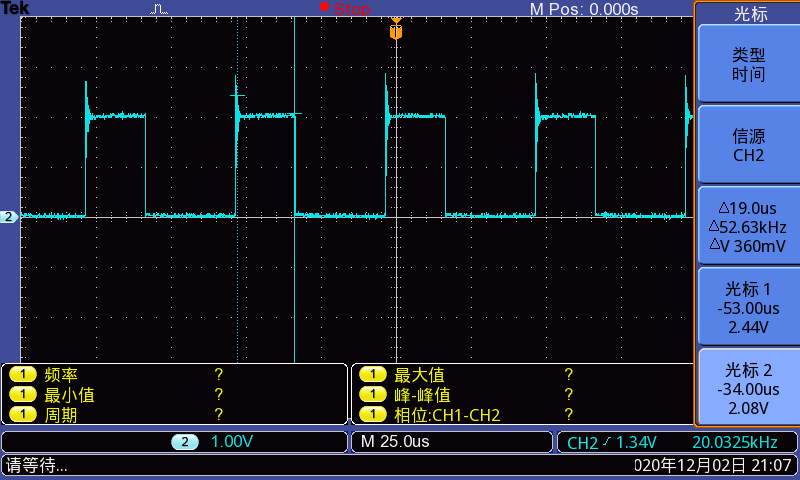
\includegraphics[
      width = \linewidth,
    ]{images/execute.png}
    \caption{执行时间}%
    \label{fig:time/execute}
  \end{subfigure}
  \quad
  \begin{subfigure}[htbp]{0.45\linewidth}
    \centering
    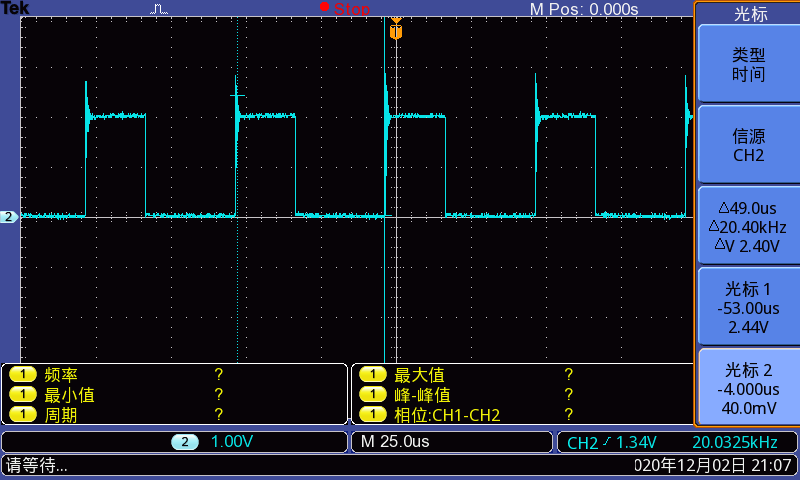
\includegraphics[
      width = \linewidth,
    ]{images/sample.png}
    \caption{采样时间}%
    \label{fig:time/sample.png}
  \end{subfigure}
  \caption{测量时间}%
  \label{fig:time}
\end{figure}

\section{实验思考}%
\label{sec:\arabic{chapter}thought}

\begin{Exercise}
  观察各种输入信号通过数字滤波器系统之后的输出波形,解释信号失真原因。
\end{Exercise}

\begin{Answer}
  选择频率 1500 Hz , 峰峰值为 1 V , 偏移为 0.5 V 的各种信号输入,输出见
  图~\ref{fig:filter},失真原因是数字滤波器会选择通带信号,衰减阻带信号。输入信
  号中阻带信号含得越多,失真越严重。
\end{Answer}

\begin{figure}[htbp]
  \centering
  \begin{subfigure}[htbp]{0.45\linewidth}
    \centering
    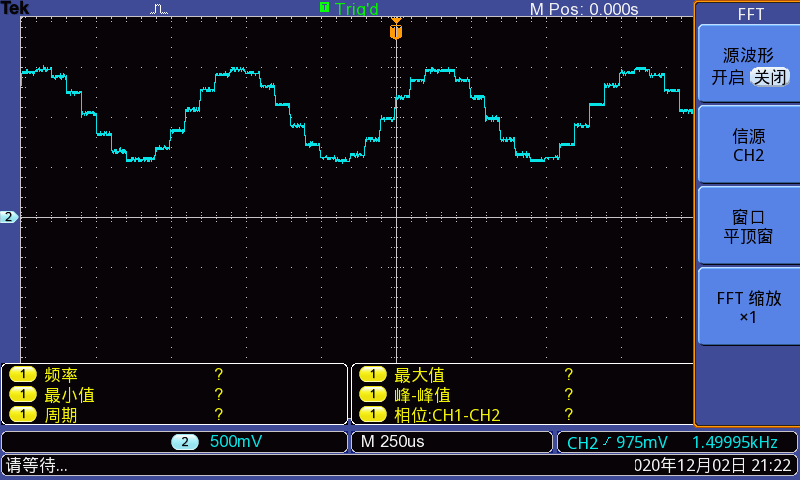
\includegraphics[
      width = \linewidth,
    ]{images/sine.png}
    \caption{正弦波}%
    \label{fig:filter/sine}
  \end{subfigure}
  \quad
  \begin{subfigure}[htbp]{0.45\linewidth}
    \centering
    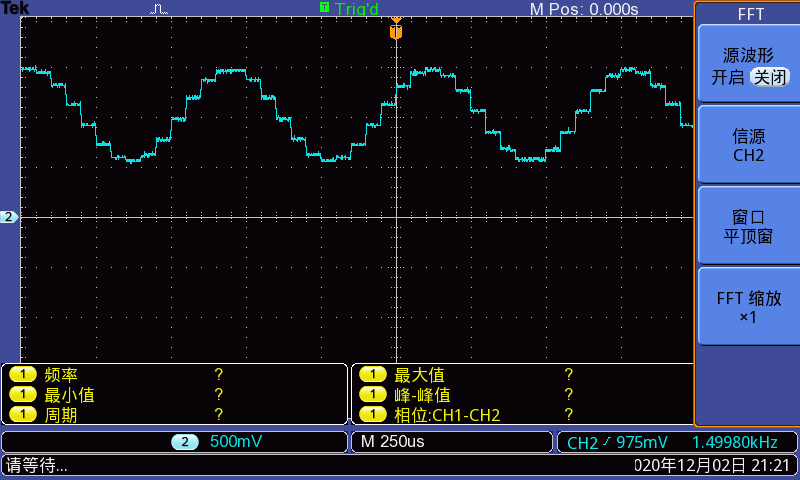
\includegraphics[
      width = \linewidth,
    ]{images/square.png}
    \caption{方波}%
    \label{fig:filter/square}
  \end{subfigure}

  \begin{subfigure}[htbp]{0.45\linewidth}
    \centering
    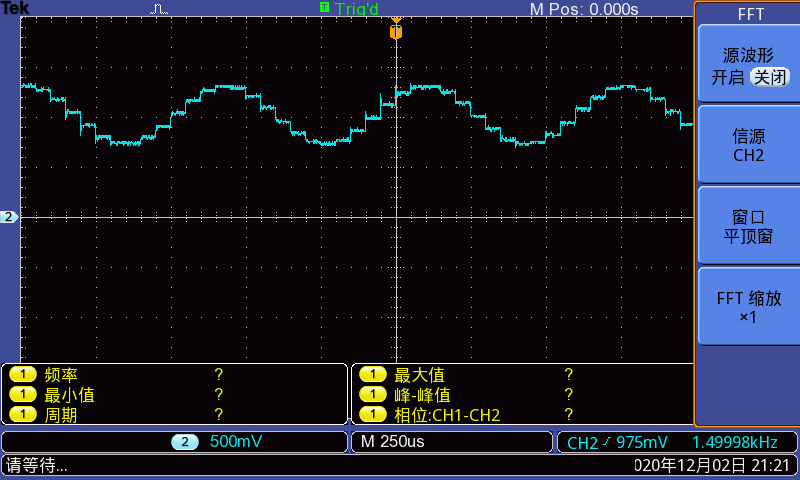
\includegraphics[
      width = \linewidth,
    ]{images/ramp.png}
    \caption{三角波}%
    \label{fig:filter/ramp}
  \end{subfigure}
  \quad
  \begin{subfigure}[htbp]{0.45\linewidth}
    \centering
    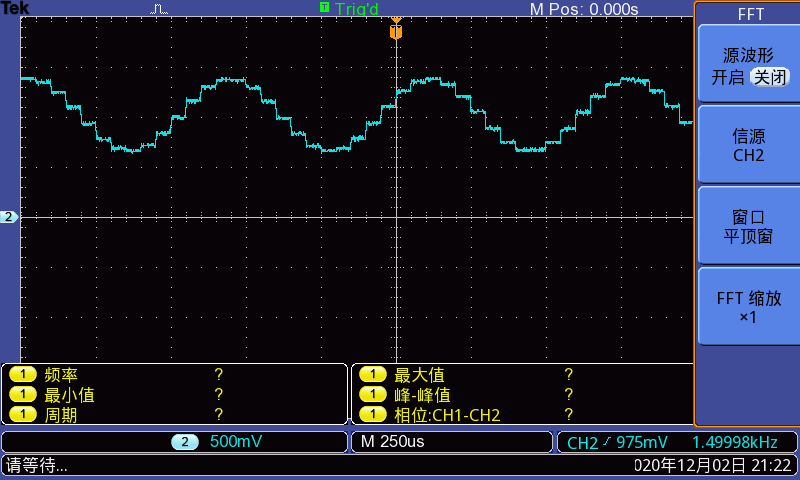
\includegraphics[
      width = \linewidth,
    ]{images/pulse.png}
    \caption{脉冲波}%
    \label{fig:filter/pulse}
  \end{subfigure}

  \begin{subfigure}[htbp]{0.45\linewidth}
    \centering
    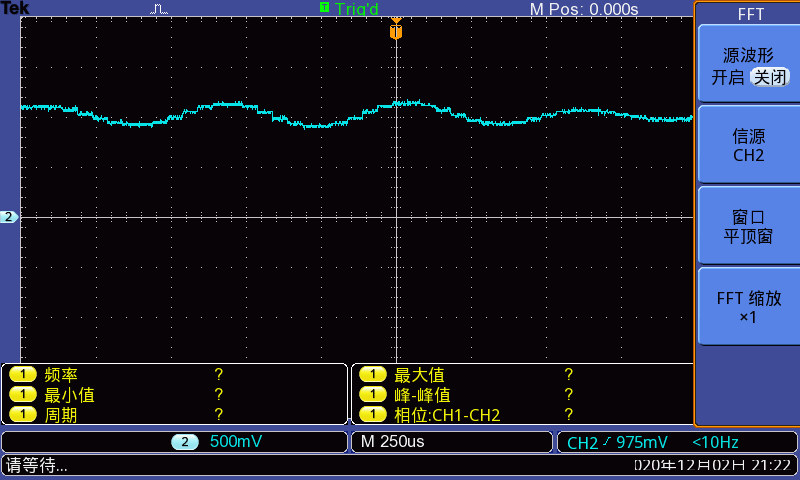
\includegraphics[
      width = \linewidth,
    ]{images/noise.png}
    \caption{噪声}%
    \label{fig:filter/noise}
  \end{subfigure}
  \quad
  \begin{subfigure}[htbp]{0.45\linewidth}
    \centering
    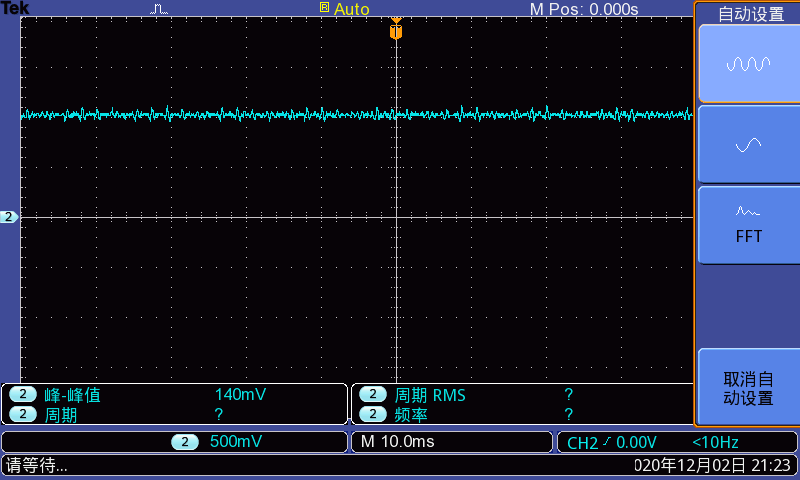
\includegraphics[
      width = \linewidth,
    ]{images/arb.png}
    \caption{心跳波}%
    \label{fig:filter/arb}
  \end{subfigure}

  \begin{subfigure}[htbp]{0.45\linewidth}
    \centering
    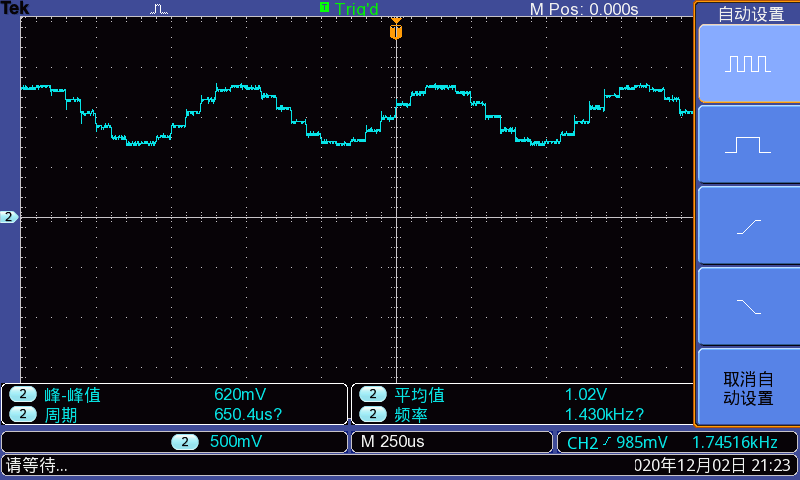
\includegraphics[
      width = \linewidth,
    ]{images/harmonic.png}
    \caption{谐波}%
    \label{fig:filter/harmonic}
  \end{subfigure}
  \quad
  \begin{subfigure}[htbp]{0.45\linewidth}
    \centering
    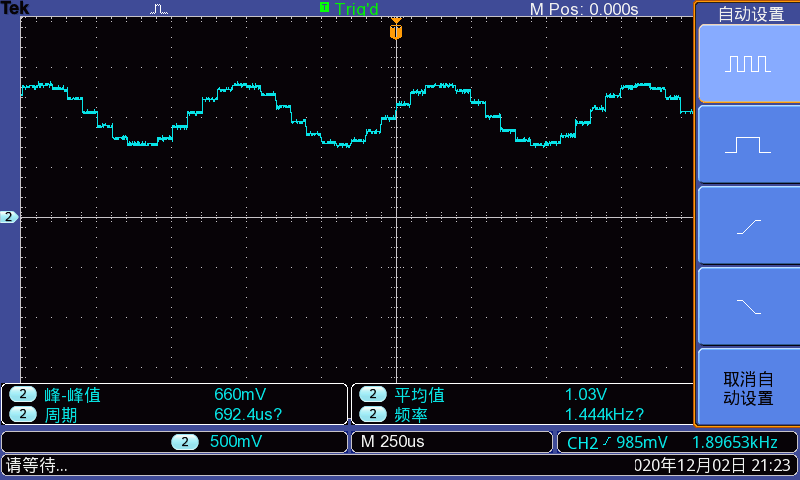
\includegraphics[
      width = \linewidth,
    ]{images/user.png}
    \caption{自定义波}%
    \label{fig:filter/user}
  \end{subfigure}
  \caption{通过数字滤波器}%
  \label{fig:filter}
\end{figure}

\begin{Exercise}
  加载由汇编语言编写的 FIR 滤波器程序,测量运算时间,比较分析 C 语言效率低的
  原因。
\end{Exercise}

\begin{Answer}
  运算时间为 2$\mu$s\footnote{实验室只有 F2812 的 FIR 汇编程序没有 F28335 的
  ,该数据来自老师称汇编语言执行时间只有 C 语言的十分之一。},因为汇编语言直
  接面向 CPU ,直接操作寄存器和存储器,节省了 C 语言抽象带来的运行开支。 C 语
  言编译后的汇编指令多达几十条,汇编语言只需要使用 2 条指令即可完成。
\end{Answer}

\begin{Exercise}
  以该 FIR 滤波器系统为例,总结分析系统实时性的取决因素。
\end{Exercise}

\begin{Answer}
  系统实时性取决于处理时间和数据输入时间的大小关系,以该 FIR 滤波器系统为例,
  因为执行时间小与采样时间,所以该系统实时。
\end{Answer}

\section{实验总结}%
\label{sec:\arabic{chapter}conclusion}

一些需要注意的地方:

\begin{itemize}
  \item 实验室的电脑和我的电脑软件版本和输出精度不同,程序~\ref{lst:fir}的结果不一样。
\end{itemize}

\end{document}

